\documentclass[10pt, a4paper]{beamer}
\usepackage{float}
\usepackage{geometry}
\usepackage{listings}
\usepackage{hyperref}
\usepackage{graphicx}
\usepackage{ragged2e}
\usepackage{color}
\usepackage{xepersian}
\usepackage{subfiles}
\usepackage{url}
\settextfont[Scale=1]{XB Roya}
\usetheme{Warsaw}
\addtobeamertemplate{navigation symbols}{}{
    \insertframenumber/\inserttotalframenumber
}

\title{گزارش توضیح‌پذیری سیستم‌های نرم‌افزاری: از آنالیز نیازمندی‌ها تا ارزیابی
سیستم}
\author{
    علیرضا سلطانی نشان
    \and 
    سودابه آشوری \\
    \and
    ملیکا محمدی گل \\
}
\institute{دانشگاه آزاد اسلامی واحد تهران شمال, خانم دکتر سپیده آدابی}


\begin{document}

\frame{\titlepage}
\begin{frame}
    \frametitle{مقدمه}

    \begin{itemize}
        \item چرایی توضیح‌پذیری
        \item قبل از توضیح‌پذیری و سپس چالش‌های آن
        \item زمینه‌گرایی توضیح
        \item اعتبارسنجی و اعتماد
    \end{itemize}
\end{frame}

\begin{frame}
    \frametitle{سابقه دانشی}

    \begin{itemize}
        \item تعاریف
        \item مدل‌ها
        \item \begin{itemize}
            \item مفهومی
            \item کیفی
            \item مرجع
        \end{itemize}
        \item راهنمای شناختی یا \lr{Catalogues}
    \end{itemize}
\end{frame}

\begin{frame}
    \frametitle{ابعاد کیفی تاثیر توضیح‌پذیری}

    \begin{figure}[H]
        \centering
        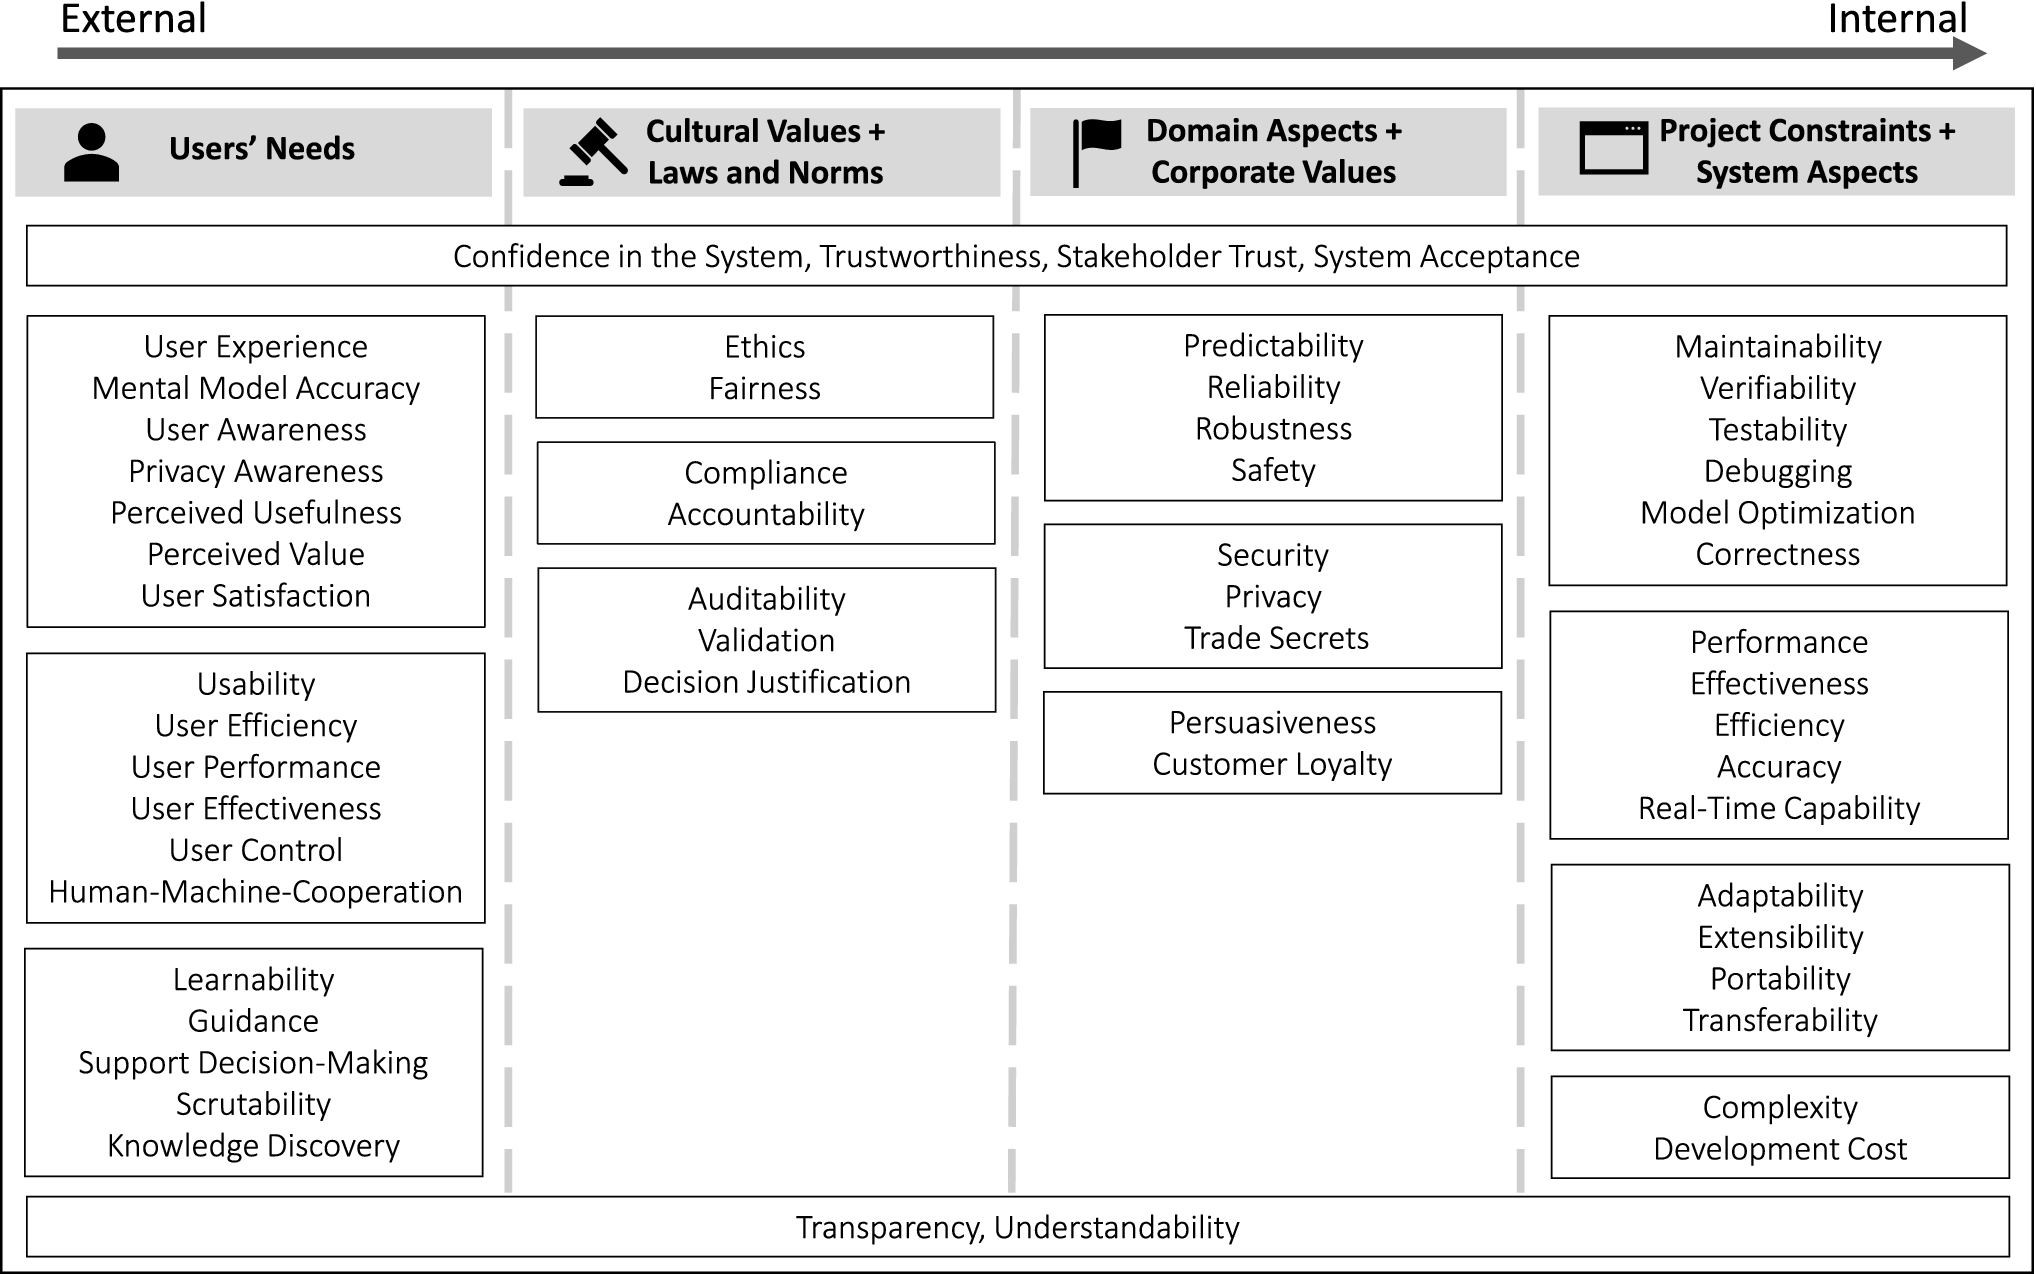
\includegraphics[width=0.9\textwidth]{images/conceptual_model.png}
        \caption{یک مدل مفهومی که تاثیر توضیح‌پذیری را در ابعاد کیفی مختلف نشان
        می‌دهد.}
        \label{fig:conceptualmodel}
    \end{figure}
\end{frame}

\begin{frame}
    \frametitle{رسالت مقاله: اهداف تحقیق و طراحی آن}
    سوال‌های پژوهشی:

    \begin{itemize}
        \item \lr{RQ1}: تعریف مناسب از توضیح‌پذیری برای رسیدن به فهم مشترک در مهندسی
        نیازمندی‌ها و مهندسی نرم‌افزار چیست؟
        \item \lr{RQ2}: حوزه‌های متاثر از توضیح‌پذیری در پس‌زمینه سیستمی چیست؟ چه
        حوزه های کیفی با توجه به زمینه سیستم (دنیای مسأله) از توضیح‌پذیری متاثر
        می‌شود؟
        \item \lr{RQ3}: چگونه توضیح‌پذیری بر سایر حوزه‌های کیفی تاثیر می‌گذارد؟
        \item \lr{RQ4}: چگونه می‌توان به متخصصان نرم‌افزار کمک کرد تا بتوانند
        فاکتورهای حائز اهمیت را در تحلیل، عملیاتی کردن و ارزیابی نیازمندی‌ها برای
        سیستم‌های توضیح‌پذیر مشخص کرد.
    \end{itemize}
\end{frame}

\begin{frame}
    \frametitle{استراتژی جست و جو در \lr{SLR} \footnote{\lr{Systematic
    Leterature Review}}}

    \begin{enumerate}
        \item جست وجوی دستی
        \item جست و جوی گلوله برفی برای تجمیع و تکمیل نتایج جست و جو
        \item \begin{itemize}
            \item \lr{Grounded Theory}
        \end{itemize}
    \end{enumerate}

    \begin{figure}[H]
        \centering
        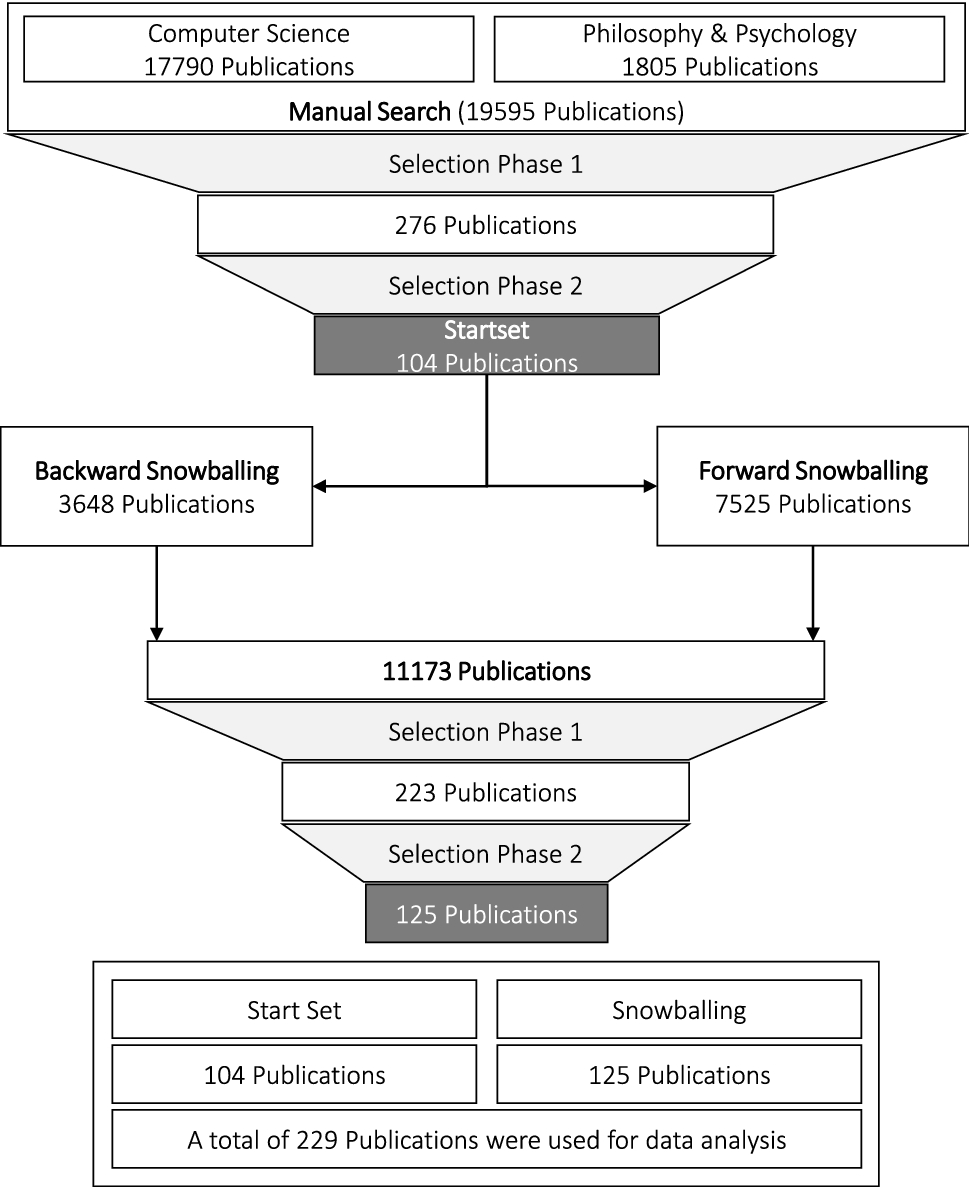
\includegraphics[width=0.3\textwidth]{images/slr_order.png}
        \caption{بررسی ساختار \lr{SLR} انجام شده در این مقاله}
        \label{fig:slrOrder}
    \end{figure}
\end{frame}

\begin{frame}
    \frametitle{دو فاز اصلی انتخاب مقالات این پژوهش}

    \begin{enumerate}
        \item انتخاب الگوریتمیک مقالات
        \item انتخاب بر مبنای ارزیابی کلی
    \end{enumerate}
\end{frame}

\begin{frame}
    \frametitle{چه فرآورده‌ای از پژوهشات انجام شده حاصل شد؟}
    دو بررسی صورت گرفت:

    \begin{enumerate}
        \item بررسی داخلی
        \item بررسی خارجی
    \end{enumerate}
\end{frame}

\begin{frame}
    \frametitle{نیازمندی‌های \lr{NFR} که در \lr{SLR} مورد بررسی قرار گرفته است:}
    ۵۷ نیازمندی غیر عملیاتی:

    \begin{figure}[H]
        \centering
    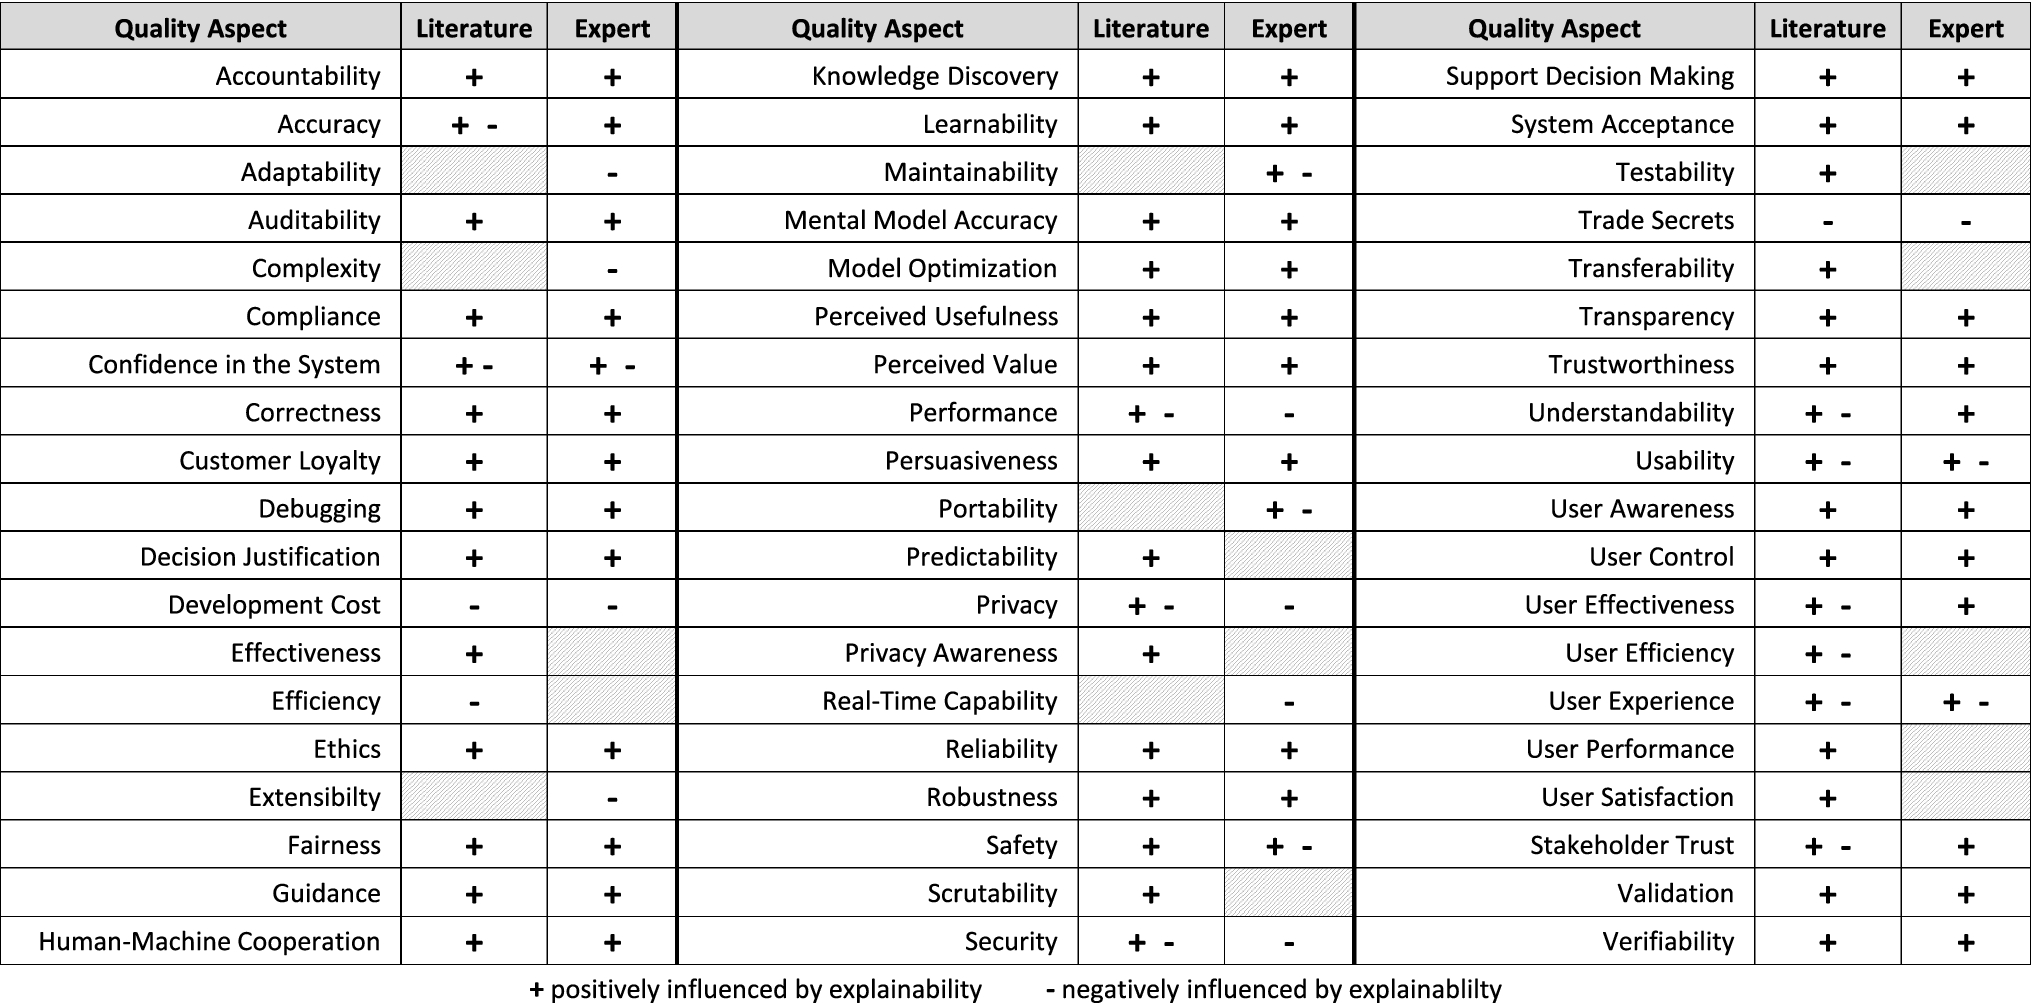
\includegraphics[width=0.9\textwidth]{images/knowledge_catalogue.png}
        \caption{راهنمای دانشی در جهت توضیح‌پذیری و تاثیر آن در جنبه‌های کیفی
        دیگر}
        \label{fig:slrOrder}
    \end{figure}
\end{frame}

\begin{frame}
    \frametitle{تاثیر ابعاد کیفی در شناسایی توضیح‌پذیری}

    \begin{itemize}
        \item اهداف
        \item محدودیت‌ها
    \end{itemize}
\end{frame}

\begin{frame}
    \frametitle{تاثیر ابعاد کیفی در شناسایی توضیح‌پذیری}

    \centering
    محدودیت‌ها باعث اعمال و شکل گرفتن تصمیمات طراحی خاص می‌شوند.
\end{frame}

\begin{frame}
    \frametitle{استراتژی پیاده‌سازی}

    \begin{itemize}
        \item توابع
        \item ماژول‌ها
        \item رابطه کاربری
    \end{itemize}
\end{frame}

\begin{frame}
    \frametitle{دو مرحله برای پیاده‌سازی}
    مبتنی بر توسعه خواهد بود:

    \begin{enumerate}
        \item مرحله پسازمان: توضیح \lr{System as is}
        \item مرحله پیش از زمان
    \end{enumerate}
\end{frame}

\begin{frame}
    \frametitle{روال استخراج اطلاعات}
    نحوه استخراج اطلاعات را برای ارائه توضیحات بررسی می‌شود:

    \centering
    "سیستم‌های مبتنی بر \lr{AI} اغلب توسط یک ماژول اضافی توضیحات خود را ارائه
    می‌دهند."
\end{frame}

\begin{frame}
    \frametitle{روال استخراج اطلاعات / سیستم‌های سنتی}

    \begin{itemize}
        \item آیا دسترسی به کد دارم؟ آیا اوپن سورس است؟
        \item الگوریتم‌ها را می‌توانم بخونم؟
        \item دسترسی به منبع داده دارم؟
        \item آیا واقعاً نیاز دسترسی مستقیم به سورس کد داریم؟ یا می‌توانیم
        داده‌ها را تحلیل کنیم؟
    \end{itemize}
\end{frame}

\begin{frame}
    \frametitle{روال استخراج اطلاعات / سیستم‌های سنتی / روش}

    \centering
    روش اختلال محلی
\end{frame}

\begin{frame}
    \frametitle{نتایج استخراج اطلاعات}

    \centering
    اینکه نتایج بدست آمده در چه زمینه‌ای است و چگونه به مخاطب و کاربرانمان آن‌ها
    را ارائه می‌دهیم امری بسیار مهم است.
\end{frame}

\begin{frame}
    \frametitle{نحوه ارائه نتایج}

    \begin{itemize}
        \item اعلام ویژگی‌هایی که مکمل یکدیگر هستند و به هم وابسته هستند.
        \item پیوند‌هایی که متناسب با توضیح مطرح می‌شوند. توضیح علتی خاص با
        ارائه مثال مناسب برای درک و فهم بهتر کاربر
    \end{itemize}
\end{frame}

\begin{frame}
    \frametitle{ارزیابی}

    \centering
    ارتباطات پلی بین اهداف کلی مشتری به یک سو و معیارهای موافقت‌ شده برای
    اندازه‌گیری به سوی دیگر می‌سازند.
\end{frame}

\begin{frame}
    \frametitle{ارزیابی}

    \begin{itemize}
        \item آیا راه‌حل‌های فنی انتخاب شده به تامین نیازمندی‌ها کمک می‌کند؟
        \item آیا در ارزیابی تاثیری دارد؟
        \item اجرای آن مطابق با انتظاراتمان بوده؟
        \item نیاز به بهبود دارد؟
    \end{itemize}
\end{frame}

\begin{frame}
    \frametitle{سطوح ارزیابی}
    حداقل دو سطح ارزیابی برای توضیح‌پذیری می‌توان در نظر گرفت:

    \begin{enumerate}
        \item ارزیابی در سطح سیستم: توضیح‌پذیری در چه جنبه‌های کیفی دیگری مشارکت
        داشته است؟
        \item ارزیابی در سطح توضیح
    \end{enumerate}
\end{frame}

\begin{frame}
    \frametitle{روش‌های ارزیابی}

    \begin{itemize}
        \item مطالعات کابری به طور کلی*
        \item پرسشنامه‌ها:"از توضیحات، من نحوه عملکرد [نرم‌افزار، الگوریتم،
        ابزار] را می‌فهمم." 
        \item آزمون‌های \lr{A/B}
        \item مطالعات موردی
        \item مصاحبه‌ها
    \end{itemize}
\end{frame}

\begin{frame}
    \frametitle{معیار‌ها}

    \begin{itemize}
        \item سازگاری
        \item پذیرفته شدن
        \item واقع‌گرایی و متقاعد‌سازی
        \item قابلیت فهم
        \item ارتباط
        \item طول (مسیر‌ها)
        \item کامل بودن یا نبودن
        \item سودمندی
    \end{itemize}

    \centering
    "یک توضیح زمانی کاربرد دارد که نه تنها جامع باشد، بلکه در لحظه‌ای مناسب مطرح
    شود تا در تصمیم‌گیری کمک کننده باشد."
\end{frame}

\begin{frame}
    \frametitle{معیار‌ها / مثال}

    \centering
    مسیریابی
\end{frame}

\begin{frame}
    \frametitle{کارگاه‌ها یا \lr{Workshops}}

    \begin{itemize}
        \item مشکلات ضمنی و راه‌حل ارائه شده
        \item آنلاین بودن کارگاه‌ها به عنوان عامل محدود‌کننده
        \item زمان اختصاص یافته کوتاه به هر کارگاه
    \end{itemize}
\end{frame}

\begin{frame}
    \centering
    جمع‌بندی نهایی
\end{frame}

\begin{frame}
    \centering
    تشکر از توجه شما
\end{frame}

\begin{frame}
    \centering
\begin{LTR}
        \centering
        \begin{figure}
            
\includegraphics[scale=0.19]{images/iau_logo.png}
        \end{figure}

        \footnotesize{Islamic Azad University - North Tehran Branch} \\
        \textbf{\footnotesize Dr.Sepideh Adabi} \\
        \small{
            Alireza Soltani Neshan - 
            Sudabeh Ashori - 
            Melika Mohammadi Gol \\
        }
        \vspace{0.3in}

        \large{Explainable Software System: From Requirements Analysis to System
        Evaluation} \\
    \end{LTR}
\end{frame}
\end{document}